%%%%%%%%%%%%%%%%%%%%%%%%%%%%%%%%%%%%%%%%%
% Short Sectioned Assignment
% LaTeX Template
% Version 1.0 (5/5/12)
%
% This template has been downloaded from:
% http://www.LaTeXTemplates.com
%
% Original author:
% Frits Wenneker (http://www.howtotex.com)
%
% License:
% CC BY-NC-SA 3.0 (http://creativecommons.org/licenses/by-nc-sa/3.0/)
%
%%%%%%%%%%%%%%%%%%%%%%%%%%%%%%%%%%%%%%%%%

%----------------------------------------------------------------------------------------
%	PACKAGES AND OTHER DOCUMENT CONFIGURATIONS
%----------------------------------------------------------------------------------------

\documentclass[paper=a4, fontsize=11pt]{scrartcl} % A4 paper and 11pt font size

\usepackage[T1]{fontenc} % Use 8-bit encoding that has 256 glyphs
\usepackage[ngerman]{babel}
\usepackage{fourier} % Use the Adobe Utopia font for the document - comment this line to return to the LaTeX default
\usepackage{amsmath,amsfonts,amsthm} % Math packages
\usepackage{graphicx}
\usepackage[utf8]{inputenc}
\usepackage{listings}
\usepackage[section]{placeins}
\usepackage{lipsum} % Used for inserting dummy 'Lorem ipsum' text into the template
\usepackage{float}
\usepackage{multicol}

\usepackage{sectsty} % Allows customizing section commands
\allsectionsfont{\centering \normalfont\scshape} % Make all sections centered, the default font and small caps

\usepackage{fancyhdr} % Custom headers and footers
\pagestyle{fancyplain} % Makes all pages in the document conform to the custom headers and footers
\fancyhead{} % No page header - if you want one, create it in the same way as the footers below
\fancyfoot[L]{} % Empty left footer
\fancyfoot[C]{} % Empty center footer
\fancyfoot[R]{\thepage} % Page numbering for right footer
\renewcommand{\headrulewidth}{0pt} % Remove header underlines
\renewcommand{\footrulewidth}{0pt} % Remove footer underlines
\setlength{\headheight}{13.6pt} % Customize the height of the header

\numberwithin{equation}{section} % Number equations within sections (i.e. 1.1, 1.2, 2.1, 2.2 instead of 1, 2, 3, 4)
\numberwithin{figure}{section} % Number figures within sections (i.e. 1.1, 1.2, 2.1, 2.2 instead of 1, 2, 3, 4)
\numberwithin{table}{section} % Number tables within sections (i.e. 1.1, 1.2, 2.1, 2.2 instead of 1, 2, 3, 4)

\setlength\parindent{0pt} % Removes all indentation from paragraphs - comment this line for an assignment with lots of text

\DeclareMathOperator*{\argmin}{arg\,min}

%----------------------------------------------------------------------------------------
%	TITLE SECTION
%----------------------------------------------------------------------------------------

\newcommand{\horrule}[1]{\rule{\linewidth}{#1}} % Create horizontal rule command with 1 argument of height

\title{
\normalfont \normalsize
\textsc{Karlsruhe Institute of Technology} \\ [25pt] % Your university, school and/or department name(s)
\horrule{0.5pt} \\[0.4cm] % Thin top horizontal rule
\huge Nichtlineare Optimierung\\ Zusammenfassung WS17/18 % The assignment title
\horrule{2pt} \\[0.5cm] % Thick bottom horizontal rule
}

\author{Manuel Lang} % Your name

\date{\normalsize\today} % Today's date or a custom date

\begin{document}

\maketitle % Print the title
%\newpage
%\tableofcontents
%\newpage

\section{Einführung}

\subsection{Begriffe}

\begin{itemize}
\item $\bar{x}$ heißt \textit{lokaler Minimalpunkt} von $f$ auf $M$, falls eine Umgebung $U$ von $\bar{x}$ mit $\forall x \in U \cap M: f(x) \ge f(\bar{x})$ existiert.
\item $\bar{x}$ heißt \textit{globaler Minimalpunkt} von $f$ auf $M$, falls man obig $U = \mathbb{R}^n$ wählen kann.
\item Ein lokaler oder globaler Minimalpunkt heißt \textit{strikt}, falls obig für $x \neq \bar{x}$ sogar die strikte Ungleichung $>$ gilt.
\item Zu jedem globalen Minimalpunkt $\bar{x}$ heißt $f(\bar{x}) (=v= \min\limits_{x \in M} f(x))$ \textit{globaler Minimalwert}, und zu jedem lokalen Minimalpunkt $\bar{x}$ heißt $f(\bar{x})$ \textit{lokaler Minimalwert}.
\item Funktion nicht differenzierbar $\implies$ nichtglattes Optimierungsproblem
\item Euklidsche Norm lässt sich durch Quadrieren (Weglassen der Wurzel) zu glattem Problem umformen (optimale Punkte bleiben erhalten)
\end{itemize}

\subsection{Lösbarkeit}

\begin{itemize}
\item $\alpha \in \mathbb{R}$ wird als \textit{untere Schranke} für $f$ auf $M$ bezeichnet, falls $\forall x \in M: \alpha \le f(x)$ gilt.
\item Das Infimum von $f$ auf $M$ ist die \textit{größte} untere Schranke von $f$ auf $M$, es gilt also $v = inf_{x \in M} f(x)$ falls $v \le f(x)$ für alle $x \in M$ gilt (d.h. $v$ ist selbst untere Schranke von $f$ auf $M$) und $\alpha \le$ für alle unteren Schranken $\alpha$ von $f$ auf $M$ gilt.
\item Definition Lösbarkeit: Das Minimierungsproblem $P$ heißt \textit{lösbar}, falls es ein $\bar{x}$ mit $inf_{x \in M} f(x) = f(\bar{x})$ existiert.
\item Satz: \textit{Das Minimierungsproblem $P$ ist genau dann lösbar, wenn es einen globalen Minimalpunkt besitzt.}
\item Satz von von Weierstraß: \textit{Die Menge $M \subseteq \mathbb{R}^n$ sei nichtleer und kompakt, und die Funktion $f: M \rightarrow \mathbb{R}$ sei stetig. Dann besitzt $f$ auf $M$ (mindestens) einen globalen Minimalpunkt und einen globalen Maximalpunkt.}
\item Definition untere Niveamenge: Für $ \subseteq \mathbb{R}^n, f:X \rightarrow \mathbb{R}$ und $\alpha \in \mathbb{R}$ heißt $lev^\alpha_\le(f,X) = \{ x \in X | f(x) \le \alpha \} $ \textit{untere Niveaumenge von $f$ auf $X$ zum Niveau $\alpha$}. Im Fall $X = \mathbb{R}^n$ schreiben wir auch kurz $f^\alpha_\le := lev^\alpha_\le (f,\mathbb{R}^n) ( = \{ x \in \mathbb{R}^n | f(x) \le \alpha \} )$.
\item Wir führen die Menge der globalen Punkte $S = \{ \bar{x} \in M | \forall x \in M: f(x) \ge f(\bar{x}) \}$ von $P$ ein.
\item Lemma: \textit{Für ein $\alpha \in \mathbb{R}$ sei $lev^\alpha_\le (f,M) \neq \emptyset$. Dann gilt $S \subseteq lev^\alpha_\le (f,M)$.}
\item Verschärfter Satz von Weierstraß: \textit{Für eine (nicht notwendiger beschränkte oder abgeschlossene) Menge $M \subseteq \mathbb{R}^n$ sei $f: M \rightarrow \mathbb{R}$ stetig, und mit einem $\alpha \in \mathbb{R}$ set $lev^\alpha_\le(f,M)$ nichtleer und kompakt. Dann besitzt $f$ auf $M$ (mindestens) einen globalen Minimalpunkt.}
\item Korollar (Verschärfter Satz von Weierstraß für unrestringierte Probleme): \textit{Die Funktion $f: \mathbb{R}^n \rightarrow \mathbb{R}$ sei stetig, und mit einem $\alpha \in \mathbb{R}$ sei $lev^\alpha_\le$ nichtleer und kompakt. Dann besitzt $f$ auf $\mathbb{R}^n$ (mindestens) einen globalen Minimalpunkt.}
\item Definition Koerzivität: Gegeben sei eine abgeschlossene Menge $X \subseteq \mathbb{R}^n$ und eine Funktion $f:X \rightarrow \mathbb{R}$. Falls für alle Folgen $(x^k) \subseteq X$ mit $lim_k ||x^k|| = +\infty$ auch $lim_k f(x^k) = + \infty$ gilt, dann heißt f \textit{koerziv} auf X.
\item Lemma: \textit{Die Funktion $f: X \rightarrow \mathbb{R}$ sei stetig und koerziv auf der (nicht notwendigerweise beschränkten) abgeschlossenen Menge $X \subseteq \mathbb{R}^n$. Dann ist die Menge $lev^\alpha_\le(f,X)$ für jedes Niveau $\alpha \in \mathbb{R}$ kompakt}.
\item Korollar: \textit{Es sei $M$ nichtleer und abgeschlossen, aber nicht allsectionsfont beschränkt. Fernser sei die Funktion $f: M \rightarrow \mathbb{R}$ stetig und koerziv auf $M$. Dann besitzt $f$ auf $M$ (mindestens) einen globalen Minimalpunkt.}
\end{itemize}

\subsection{Rechenregeln und Umformungen}

\begin{itemize}
\item Skalare Vielfache und Summen
\begin{itemize}
\item $\forall \alpha \ge 0, \beta \in \mathbb{R}$: $min_{x \in M} (\alpha f(x) + \beta) = \alpha (min_{x \in M} f(x)) + \beta$.
\item $\forall \alpha \le 0, \beta \in \mathbb{R}$: $min_{x \in M} (\alpha f(x) + \beta) = \alpha (max_{x \in M} f(x)) + \beta$.
\item $min_{x \in M} (f(x) + g(x)) \ge min_{x \in M} f(x) + min_{x \in M} g(x)$.
\item In obiger Ungleichung kann der strikte Fall $>$ auftreten.
\item In den ersten beiden Zeilen stimmen die lokalen bzw. globalen Optimalpunkte der Optimierungsprobleme überein.
\end{itemize}
\item Separable Zielfunktion auf kartesischem Punkt
\begin{itemize}
\item Es seien $X \subseteq \mathbb{R}^n, Y \subseteq \mathbb{R}^m, f: X \rightarrow \mathbb{R}$ und $g: Y \rightarrow \mathbb{R}$. Dann gilt $\min\limits_{(x,y)\in X x Y} (f(x) + g(y)) = \min\limits_{x \in X} f(x) + \min\limits_{y \in Y} g(y)$
\end{itemize}
\item Vertauschung von Minima und Maxima
\begin{itemize}
\item Es seien $X \subseteq \mathbb{R}^n, Y \subseteq \mathbb{R}^m, M = X x Y$ und $f: M \rightarrow \mathbb{R}$ gegeben. Dann gilt:
\item $min_{(x,y)\in M}f(x,y) = min_{x \ in X} min_{y \in Y} f(x,y) = min_{y \in Y} min_{x \in X} f(x,y)$.
\item $max_{(x,y)\in M}f(x,y) = max_{x \ in X} max_{y \in Y} f(x,y) = max_{y \in Y} max_{x \in X} f(x,y)$.
\item $min_{x \in X} max_{y \in Y} f(x,y) \ge max_{y \in Y} min_{x \in X} f(x,y)$.
\item In obiger Ungleichung kann der strikte Fall $>$ auftreten.
\end{itemize}
\item Monotone Transformation: Zu $M \subseteq \mathbb{R}^n$ und einer Funktion $f: M \rightarrow Y$ mit $Y \subseteq \mathbb{R}$ sei $\psi : Y \rightarrow \mathbb{R}$ eine streng monoton wachsende Funktion. Dann gilt $\min\limits_{x \in M} \psi(f(x)) = \psi(\min\limits_{x \in M} f(x))$, und die lokalen bzw. globalen Minimalpunkte stimmen überein.
\item Epigrahumformulierung: Gegeben seien $M \subseteq \mathbb{R}^n$ und eine Funktion $f: M \mathbb{R}$. Dann sind die Probleme $P: \min\limits_{x \in \mathbb{R}^n} f(x)$ s.t. $x \in M$ und $P_{epi}: \min\limits_{x,\alpha \in \mathbb{R}^n x \mathbb{R}} \alpha$ s.t. $f(x) \le \alpha, x \in M$ in folgendem Sinne äquivalent.
\begin{itemize}
\item Für jeden lokalen bzw. globalen Minimalpunkt $x^*$ von $P$ ist $(x^*,f(x^*))$ lokaler bzw. globaler Minimalpunkt von $P_{epi}$.
\item Für jeden lokalen bzw. globalen Minimalpunkt $(x^*,\alpha^*)$ von $P_{epi}$ ist $x^*$ lokaler bzw. globaler Minimalpunkt von $P$.
\item Die Minimalwerte von $P$ und $P_{epi}$ stimmen überein.
\end{itemize}
\item Definition Parallelprojektion: Es sei $M \subseteq \mathbb{R}^n x \mathbb{R}^m$. Dann heißt $pr_x M = \{ x \in \mathbb{R}^n | \exists y \in \mathbb{R}^m : (x,y) \in M \}$ Parallelprojektion von $M$ auf den \glqq x-Raum \grqq $\mathbb{R}^n$.
\item Projektionsumformulierung: Gegeben seien $M \subseteq \mathbb{R}^n x \mathbb{R}^m$ und eine Funktion $f: \mathbb{R}^n \rightarrow \mathbb{R}$, die nicht von den Variablen aus $\mathbb{R}^m$ abhängt. Dann sind die Probleme $P: \min\limits_{(x,y) \in \mathbb{R}^n x \mathbb{R}^m} f(x)$ s.t. $(x,y) \in M$ und $P_{proj}: \min\limits_{x \in \mathbb{R}^n} f(x)$ s.t. $x \in pr_x M$ in folgendem Sinne äquivalent:
\begin{itemize}
\item Für jeden lokalen bzw. globalen Minimalpunkt $(x^*,y^*)$ von $P$ ist $x^*$ lokaler bzw. globaler Minimalpunkt von $P_{proj}$.
\item Für jeden lokalen bzw. globalen Minimalpunkt $x^*$ von $P_{proj}$ existiert ein $y^* \in \mathbb{R}^n$, sodass $(x^*,y^*)$ lokaler bzw. globaler Minimalpunkt von $P$ ist.
\item Die Minimalwerte von $P$ und $P_{proj}$ stimmen überein.
\end{itemize}
\end{itemize}

\section{Unrestringierte Optimierung}

\subsection{Optimalitätsbedingungen}

\subsubsection{Abstiegsrichtungen}

\begin{itemize}
\item Definition Abstiegsrichtung: Es seien $f: \mathbb{R}^n \rightarrow \mathbb{R}$ und $\bar{x} \in \mathbb{R}^n$. Ein Vektor $d \in \mathbb{R}^n$ heißt \textit{Abstiegsrichtung} für $f$ in $\bar{x}$ falls $\exists \check{t} > 0 \forall t \in (0, \check{t}): f(\bar{x} + td) < f(\bar{x})$ gilt.
\item Definition eindimensionale Einschränkung: Gegeben seien $f: \mathbb{R}^n \rightarrow \mathbb{R}$, ein Punkt $\bar{x} \in \mathbb{R}^n$ und ein Richtungsvektor $d \in \mathbb{R}^n$. Die Funktion $\phi_d : \mathbb{R}^1 \rightarrow \mathbb{R}^1, t 	\mapsto f(\bar{x} + td)$ heißt \textit{eindimensionale Einschränkung} von $f$ auf die durch $\bar{x}$ in Richtung $d$ verlaufende Gerade.\\
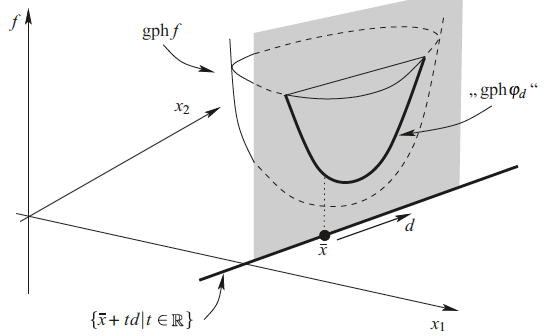
\includegraphics[width=0.5\textwidth]{imgs/eindimeinschr}
\end{itemize}

\subsubsection{Optimimalitätsbedingung erster Ordnung}

\begin{itemize}
\item Definition einseitige Richtungsbleitung: Eine Funktion $f : \mathbb{R}^n \rightarrow \mathbb{R}$ heißt an $\bar{x} \in \mathbb{R}^n$ in eine Richtung $d \in \mathbb{R}^n$ \textit{einseitig richtungsdifferenzierbar}, wenn der Grenzwert $f'(\bar{x},d) := \lim\limits_{t \searrow 0} \frac{f(\bar{x} + td) - f(\bar{x})}{t}$ existiert. Der Wert $f'(\bar{x},d)$ heißt dann \textit{einseitige Richtungsableitung}. Die Funktion $f$ heißt an $\bar{x}$ \textit{einseitig richtungsdifferenzierbar}, wenn $f$ an $\bar{x}$ in jede Richtung $d \in \mathbb{R}^n$ einseitung richtungsdifferenzierbar ist, und $f$ heißt \textit{einseitig richtungsdifferenzierbar}, wenn $f$ an jedem $\bar{x} \in \mathbb{R}^n$ einseitig richtungsdifferenzierbar ist.
\item Lemma: Die Funktion $f: \mathbb{R}^n \rightarrow R$ sei an $\bar{x} \in \mathbb{R}^n$ in Richtung $d \in \mathbb{R}^n$ einseitig richtungsdifferenzierbar mit $f'(\bar{x},d) < 0$. Dann ist $d$ Abstiegsrichtung für $f$ in $\bar{x}$.
\item Lemma: Die Funktion $f: \mathbb{R}^n \rightarrow \mathbb{R}$ sei an einem lokalen Minimalpunkt $\bar{x} \in \mathbb{R}^n$ einseitig richtungsdifferenzierbar. Dann gilt $f'(\bar{x},d) \ge 0$ für jede Richtung $d \in \mathbb{R}^n$.
\item Definition Abstiegsrichtung erster Ordnung: Für eine am Punkt $\bar{x} \in \mathbb{R}^n$ in Richtung $d \in \mathbb{R}^n$ einseitig richtungsdifferenzierbare Funktion $f: \mathbb{R}^n \rightarrow \mathbb{R}$ heißt $d$ \textit{Abstiegsrichtung erster Ordnung}, falls $f'(\bar{x},d) < 0$ gilt.
\item Definition stationärer Punkt: Die Funktion $f: \mathbb{R}^n \rightarrow \mathbb{R}$ sei an $\bar{x} \in \mathbb{R}^n$ einseitig richtungsdifferenzierbar. Dann heißt $\bar{x}$ \textit{stationärer Punkt} von $f$, falls $f'(\bar{x},d) \ge 0$ für jede Richtung $d \in \mathbb{R}^n$ gilt.
\item Als \textit{erste Ableitung} einer partiell differenzierbaren Funktion $f: \mathbb{R}^n \rightarrow \mathbb{R}$ an $\bar{x}$ betrachtet man den Zeilenvektor $Df(\bar{x}) := (\partial_{x_1}f(\bar{x}), ..., \partial_{x_n}f(\bar{x}))$ oder auch sein Transponiertes $\nabla f(\bar{x}) := (Df(\bar{x}))^T$.
\item Für eine vektorwertige Funktion $f: \mathbb{R}^n \rightarrow \mathbb{R}^m$ mit partiell differenzierbaren Komponenten $f_1, ..., f_m$ definiert man die erste Ableitung als $Df(\bar{x}) := \begin{pmatrix}
Df_1(\bar{x}) \\
\vdots \\
Df_m(\bar{x})
\end{pmatrix} $. Diese $(m,n)$-Matrix heißt \textit{Jacobi-Matrix} oder \textit{Funktionalmatrix} von $f$ an $\bar{x}$.
\item Satz Kettenregel: Es seien $g: \mathbb{R}^n \rightarrow \mathbb{R}^m$ differenzierbar an $\bar{x} \in \mathbb{R}^n$ und $f: \mathbb{R}^m \rightarrow \mathbb{R}^k$ differenzierbar an $g(\bar{x}) \in \mathbb{R}^m$. Dann ist $f \circ g: \mathbb{R}^n \rightarrow \mathbb{R}^k$ differenzierbar an $\bar{x}$ mit $D(f \circ g)(\bar{x}) = Df(g(\bar{x})) \cdot Dg(\bar{x})$.
\item Bei der Anwendung der Kettenregel auf die Funktion $\phi_d(t) = f(\bar{x} + t d)$ gilt $k = m = 1$ und $g(t) = \bar{x} + td$. Als Jacobik-Matrix von $g$ erhält man $Dg(t) = d$ und damit $\phi'_d(0) = Df(\bar{x}) d$. Das Matrixprodukt aus der Kettenregel wird in diesem Spezialfall also zum Produkt des Zeilenvektors $Df(\bar{x})$ mit dem Spaltenvektor $d$. Für zwei allgemeine (Spalten-) Vektoren $a,b \in \mathbb{R}^n$ nennt man den so definierten Term $a^T b = \sum\limits_{i=1}^n a_i b_i$ auch (Standard-) Skalarprodukt von $a$ und $b$. Eine alternative Schreibweise dafür ist $\langle a,b\rangle := a^T b$. Wir erhalten also $\phi'_d(0) = \langle \nabla f(\bar{x}),d\rangle$ und können damit zunächst Lemma 2.1.5 umformulieren.
\item Lemma 2.1.10: Die Funktion $f: \mathbb{R}^n \rightarrow \mathbb{R}$ sei am Punkt $\bar{x} \in \mathbb{R}^n$ differenzierbar, und für die Richtung $d \in \mathbb{R}^n$ gelte $\langle f(\bar{x}),d \rangle < 0$. Dann ist $d$ Abstiegsrichtung für $f$ in $\bar{x}$.
\item Für zwei Vektoren $a,b \in \mathbb{R}^n$ besitzt das Skalarprodukt $\langle a,b \rangle$ neben der algebraischen Definition zu $a^T b$ auch die geometrische Darstellung $\langle a,b \rangle = ||a||_2 \cdot ||b||_2 \cdot cos(\angle(a,b))$.
\item Satz 2.1.13 Notwendige Optimalitätsbedingung erster Ordnung - Fermat'sche Regel: Die Funktion $f: \mathbb{R}^n \rightarrow \mathbb{R}$ sei differenzierbar an einem lokalen Minimalpunkt $\bar{x} \in \mathbb{R}^n$. Dann gilt $\nabla f(\bar{x}) = 0$.
\item Die Fermat'sche Regel wird als \textit{Optimalitätsbedingung erster Ordnung} bezeichnet, da sie von der ersten Ableitung der Funktion $f$ Gebrauch macht. Sie motiviert die folgende Definition.
\item Definition kritischer Punkt: Die Funktion $f: \mathbb{R}^n \rightarrow \mathbb{R}$ sei an $\bar{x} \in \mathbb{R}^n$ differenzierbar. Dann heißt $\bar{x}$ \textit{kritischer Punkt} von $f$, wenn $\nabla f(\bar{x})$ gilt.
\item In dieser Terminologie ist nach der Fermat'schen Regel jeder lokale Minimalpunkt einer differenzierbaren Funktion notwendingerweise kritischer Punkt.
\item Definition Sattelpunkt: Die Funktion $f: \mathbb{R}^n \rightarrow \mathbb{R}$ sei an $\bar{x} \in \mathbb{R}^n$ differenzierbar. Dann heißt $\bar{x}$ \textit{Sattelpunkt} von $f$, falls $\bar{x}$ zwar kritischer Punkt von $f$, aber weder lokaler Minimal- noch Maximalpunkt ist.
\item Da die Fermat'sche lediglich eine notwendige, nicht aber eine hinreichende Bedingung ist, sind kritische Punkt lediglich Kandidaten für Minimalpunkt von $f$, können aber auch Maximal- oder Sattelpunkten entsprechen.
\end{itemize}

\subsubsection{Geometrische Eigenschaften von Gradienten}

\begin{itemize}
\item Um die geometrische Interpretation des Gradienten $\nabla f(\bar{x})$ vollzuständig zu verstehen, bringen wir ihn mit der unteren Niveaumenge $f^{f(\bar{x})}_\le = \{ x \in \mathbb{R}^n | f(x) \le f(\bar{x}) \}$ in Verbindung. Sie ist für Minimierungsverfahren von grundlegender Bedeutung, da einerseits offensichtlich $\bar{x} \in f^{f(\bar{x})}_\le$ gilt und im Vergleich zu $\bar{x}$ \glqq bessere \grqq\ Punkte $x$ gerade solche sind, die die strikte Ungleichung $f(x) < f(\bar{x})$ erfüllen.
\item Cauchy-Schwarz-Ungleichgung: $- ||\nabla f(\bar{x})||_2 = - || \nabla f(\bar{x}) ||_2 \le \langle f(\bar{x}),d \rangle \le ||\nabla f(\bar{x}) ||_2 \cdot ||d||_2 = ||\nabla f(\bar{x}) ||_2$
\item Die kleinstmögliche Steigung $-||\nabla f(\bar{x})||_2$ wird wegen $\nabla f(\bar{x}) \neq 0$ mit $d = - \frac{\nabla f(\bar{x})}{||\nabla f(\bar{x})||_2}$ realisiert und die größtmögliche $+ ||\nabla f(\bar{x})||_2$ mit $d = + \frac{\nabla f(\bar{x})}{||\nabla f(\bar{x})||_2}$.
\item Insbesondere entspricht die Länge $||\nabla f(\bar{x})||_2$ des Gradienten genau dem größtmöglichen Anstieg der Funktion $f$ von $\bar{x}$ aus, und die Richtung des Gradienten zeigt in die zugehörige Richtung des steilsten Anstiegs.
\end{itemize}

\subsubsection{Optimalitätsbedingungen zweiter Ordnung}

\begin{itemize}
\item univariat = betrachtete Funktion hängt nur von einer Variablen ab
\item Satz 2.1.19 (Entwicklungen erster und zweiter Ordnung per univariatem Satz von Taylor)
\begin{itemize}
\item Es sei $\phi: \mathbb{R} \rightarrow \mathbb{R}$ differenzierbar an $\bar{t}$. Dann gilt für alle $t \in \mathbb{R}$: $\phi(t) = \phi(\bar{t}) + \phi'(\bar{t})(t-\bar{t}) + o(|t-\bar{t}|)$, wobei $o(|t-\bar{t}|)$ einen Ausdruck der Form $\omega(t) \cdot |t-\bar{t}|$ mit $lim_{t \rightarrow \bar{t}} \omega(t) = w(\bar{t}) = 0$ bezeichnet.
\item Es sei $\phi: \mathbb{R} \rightarrow \mathbb{R}$ zweimal differenzierbar an $\bar{t}$. Dann gilt für alle $t \in \mathbb{R}$: $\phi(t) = \phi(\bar{t}) + \phi'(\bar{t})(t-\bar{t}) + \frac{1}{2} \phi''(\bar{t})(t-\bar{t})^2 + o(|t-\bar{t}|^2)$, wobei $o(|t-\bar{t}|^2)$ einen Ausruck der Form $\omega(t) \cdot |t-\bar{t}|^2$ mit $lim_{t \rightarrow \bar{t}} \omega(t) = w(\bar{t}) = 0$ bezeichnet.
\end{itemize}
\item Lemma 2.1.20: Für $f: \mathbb{R}^n \rightarrow \mathbb{R}$, einen Punkt $\bar{x} \in \mathbb{R}^n$ und eine Richtung $d \in \mathbb{R}^n$ seien $\phi'_d(0) = 0$ und $\phi''_d(0) < 0$. Dann ist $d$ Abstiegsrichtung für $f$ in $\bar{x}$.
\item Lemma 2.1.21: Für $f: \mathbb{R}^n \rightarrow \mathbb{R}$ sei $\bar{x}$ ein lokaler Minimalpunkt. Dann gilt $\nabla(\bar{x}) = 0$, und jede Richtung $d \in \mathbb{R}^n$ erfüllt $\phi''_d(0) \ge 0$.
\item Die $(n,n)$-Matrix $D^2f(\bar{x}) := D\nabla f(\bar{x}) = := \begin{pmatrix}
\partial_{x_1} \partial_{x_1} f(\bar{x}) & \cdots & \partial_{x_n} \partial_{x_1} f(\bar{x})\\
\vdots & & \vdots\\
\partial_{x_1} \partial_{x_n} f(\bar{x}) & \cdots & \partial_{x_n} \partial_{x_n} f(\bar{x})
\end{pmatrix} $ heißt \textit{Hesse}-Matrix von $f$ an $\bar{x}$. Als zweite Ableitung sind in ihr Krümmungsinformationen von $f$ and $\bar{x}$ codiert.
\item Lemma 2.1.22: Für $f: \mathbb{R}^n \rightarrow \mathbb{R}$, einen Punkt $\bar{x} \in \mathbb{R}^n$ und eine Richtung $d \in \mathbb{R}^n$ seien $\langle \nabla f(\bar{x}),d \rangle = 0$ und $d^T D^2f(\bar{x})d < 0$. Dann ist §d§ Abstiegsrichtung für $f$ in $\bar{x}$.
\item Definition Abstiegsrichtung zweiter Ordnung: Zu $f: \mathbb{R}^n \rightarrow \mathbb{R}$ und $\bar{x} \in \mathbb{R}^n$ heißt jeder Richtungsvektor $d \in \mathbb{R}^n$ mit $\langle \nabla f(\bar{x}), d \rangle = 0$ und $d^T D^2f(\bar{x})d < 0$ Abstiegsrichtung zweiter Ordnung für $f$ in $\bar{x}$.
\item Satz 2.1.27 Notwendige Optimalitätsbedingung zweiter Ordnung: Die Funktion $f: \mathbb{R}^n \rightarrow \mathbb{R}$ sei zweimal differenzierbar an einem lokalen Minimalpunkt $\bar{x} \in \mathbb{R}^n$. Dann gilt $\nabla f(\bar{x}) = 0$ und $D^2f(\bar{x}) \ge 0$.
\item Eine symmetrische Matrix ist genau dann positiv semidefinit, wenn ihre sämtlichen Eigenwerte nichtnegativ sind.
\item Demnach dürfen wir für jede $C^2$-Funktion (zwei mal stetig differenzierbar) $f$ die Bedingung $D^2f(\bar{x}) \ge 0$ verifizieren, indem wir die $n$ Eigenwerte der Matrix $D^2f(\bar{x})$ berechnen und auf Nichtnegativität überprüfen.
\item Positive Definitheit bedeutet, dass alle Eigenwerte von $D^2f(\bar{x})$ strikt positiv sind.
\item Satz 2.1.30 Enticklungen erster und zweiter Ordnung per multivariatem Satz von Taylor
\begin{itemize}
\item Es sei $f: \mathbb{R}^n \rightarrow \mathbb{R}$ differenzierbar in $\bar{x}$. Dan gilt für alle $x \in \mathbb{R}^n$: $f(x) = f(\bar{x}) + \langle \nabla f(\bar{x}), x - \bar{x} \rangle + o(||x-\bar{x})||$, wobei $o(||x-\bar{x})||$ einen Ausdruck der Form $\omega(x) \cdot ||x-\bar{x}|| mit lim_{x \rightarrow \bar{x}} \omega{x} = \omega{\bar{x}} = 0$ bezeichnet.
\item Es sei $f: \mathbb{R}^n \rightarrow \mathbb{R}$ zweimal differenzierbar in $\bar{x}$. Dann gilt für alle $x \in \mathbb{R}^n$: $f(x) = f(\bar{x}) + \langle \nabla f(\bar{x}),x-\bar{x} \rangle + \frac{1}{2}(x-\bar{x})^T D^2f(\bar{x})(x-\bar{x}) + o(||x-\bar{x}||^2)$, wobei $o(||x-\bar{x}||^2)$ einen Ausruck der Form $\omega(x) \cdot ||x-\bar{x}||^2$ mit $lim_{x \rightarrow \bar{x}} \omega(x) = \omega()\bar{x}) = 0$ bezeichnet.
\end{itemize}
\item Satz 2.1.31 Hinreichende Optimalitätsbedingung zweiter Ordnung: Die Funktion $f: \mathbb{R}^n \rightarrow \mathbb{R}$ sei an $\bar{x} \in \mathbb{R}$ zweimal differenzierbar, und es gelte $\nabla f(\bar{x}) = 0$ und $D^2f(\bar{x}) \succ 0$. Dann ist $\bar{x}$ ein strikter lokaler Minimalpunkt von $f$.
\item Definition 2.1.35 Nichtdegenerierte kritische und Minimalpunkte: Die Funktion $f: \mathbb{R}^n \rightarrow \mathbb{R}$ sei an $\bar{x}$ zweimal differenzierbar mit $\nabla f(\bar{x}) = 0$. Dann heißt $\bar{x}$
\begin{itemize}
\item nichtdegenerierter kritischer Punkt, falls $D^2f(\bar{x})$ nichsingulär ist,
\item nichtdegenerierter lokaler Minimalpunkt, falls $\bar{x}$ lokaler Minimalpunkt und nichtdegenerierter kritischer Punkt ist.
\end{itemize}
\item Lemma 2.1.36: Der Punkt $\bar{x}$ ist genau dann nichtdegenerierter lokaler Minimalpunkt von $f$, wenn $\nabla f(\bar{x}) = 0$ und $D^2f(\bar{x}) \succ 0$ gilt.
\item Wir definieren $\mathcal{F} = \{  f \in C^2(\mathbb{R}^n,\mathbb{R}) |$ alle kritischen Punkte von $f$ sind nichtdegeneriert $\}$
\item Satz 2.1.37: $\mathcal{F}$ ist $C^2_s$-offen und -dicht in $C^2(\mathbb{R}^n,\mathbb{R})$.
\end{itemize}

\subsubsection{Konvexe Optimierungsprobleme}

\begin{itemize}
\item Definition konvexe Menge und Funktionen
\begin{itemize}
\item Eine Menge $X \subseteq \mathbb{R}^n$ heißt konvex, falls $\forall x,y \in X, \lambda \in (0,1): (1-\lambda)x + \lambda y \ in X$ gilt (d.h. die Verbindungsstrecke von je zwei beliebigen Punkten in $X$ gehört komplett zu $X$.)
\item Für eine konvexe Menge $X \subseteq \mathbb{R}^n$ heißt eine Funktion $f: X \rightarrow \mathbb{R}$ konvex (auf $X$), falls $\forall x,y \in X, \lambda \in (0,1): f((1-\lambda)x+\lambda y) \le (1-\lambda)f(x) + \lambda f(y)$ gilt (d.h. der FUnktionsgraph von $f$ verläuft unter jeder seiner Sekanten).
\end{itemize}
\item Satz 2.1.40 $C^1$-Charakterisierung von Konvexität: Auf einer konvexen Menge $X \subseteq \mathbb{R}^n$ ist eine Funktion $f \in C^1(X,\mathbb{R})$ genau dann konvex, wenn $\forall x,y \in X: f(y) \ge f(x) + \langle \nabla f(x),y-x\rangle$ gilt.
\item Korollar 2.1.41: Die Funktion $f \in C^1(\mathbb{R}^n,\mathbb{R})$ sei konvex. Dann sind die kritischen Punkte von $f$ genau die globalen Minimalpunkt von $f$.
\item Satz 2.1.42 $C^2$-Charakterisierung von Konvexität: Eine Funktion $f \in C^2(\mathbb{R}^n,\mathbb{R})$ ist genau dann konvex, wenn $\forall x \in \mathbb{R}^n: D^2f(x) \ge 0$ gilt.
\end{itemize}

\end{document}
